\pagebreak
\section{SOP: Reidentification}
\label{section:sop_reidentification}

\par\noindent\rule{\textwidth\color{pniblue}}{0.4pt}
\subsection*{Step 1. Obtaining the long ID}
\addcontentsline{toc}{subsubsection}{Obtaining the long ID}

If the re-identification (i.e. obtaining the personal data of a participant given the pseudonym, e.g. in case of incidental findings) is needed the first task is to obtain the long ID, based on the short ID.
This can usually be achieved by a query of the merged dataset, resulting from data consolidation (see section \ref{section:overview}). Alternatively, the researcher is also able to obtain this information by logging in into the LimeSurvey web application (see Step 1 in section \ref{section:ls_setup}), navigating to the participant table of a survey the participant was involved in (see 'Information about further use of the surveys' in section \ref{section:ls_setup}), and searching for the correct long-short ID pair as shown on the figure below.
Copy the long ID to the clipboard (selection then Ctr+C).

\begin{figure}[H]
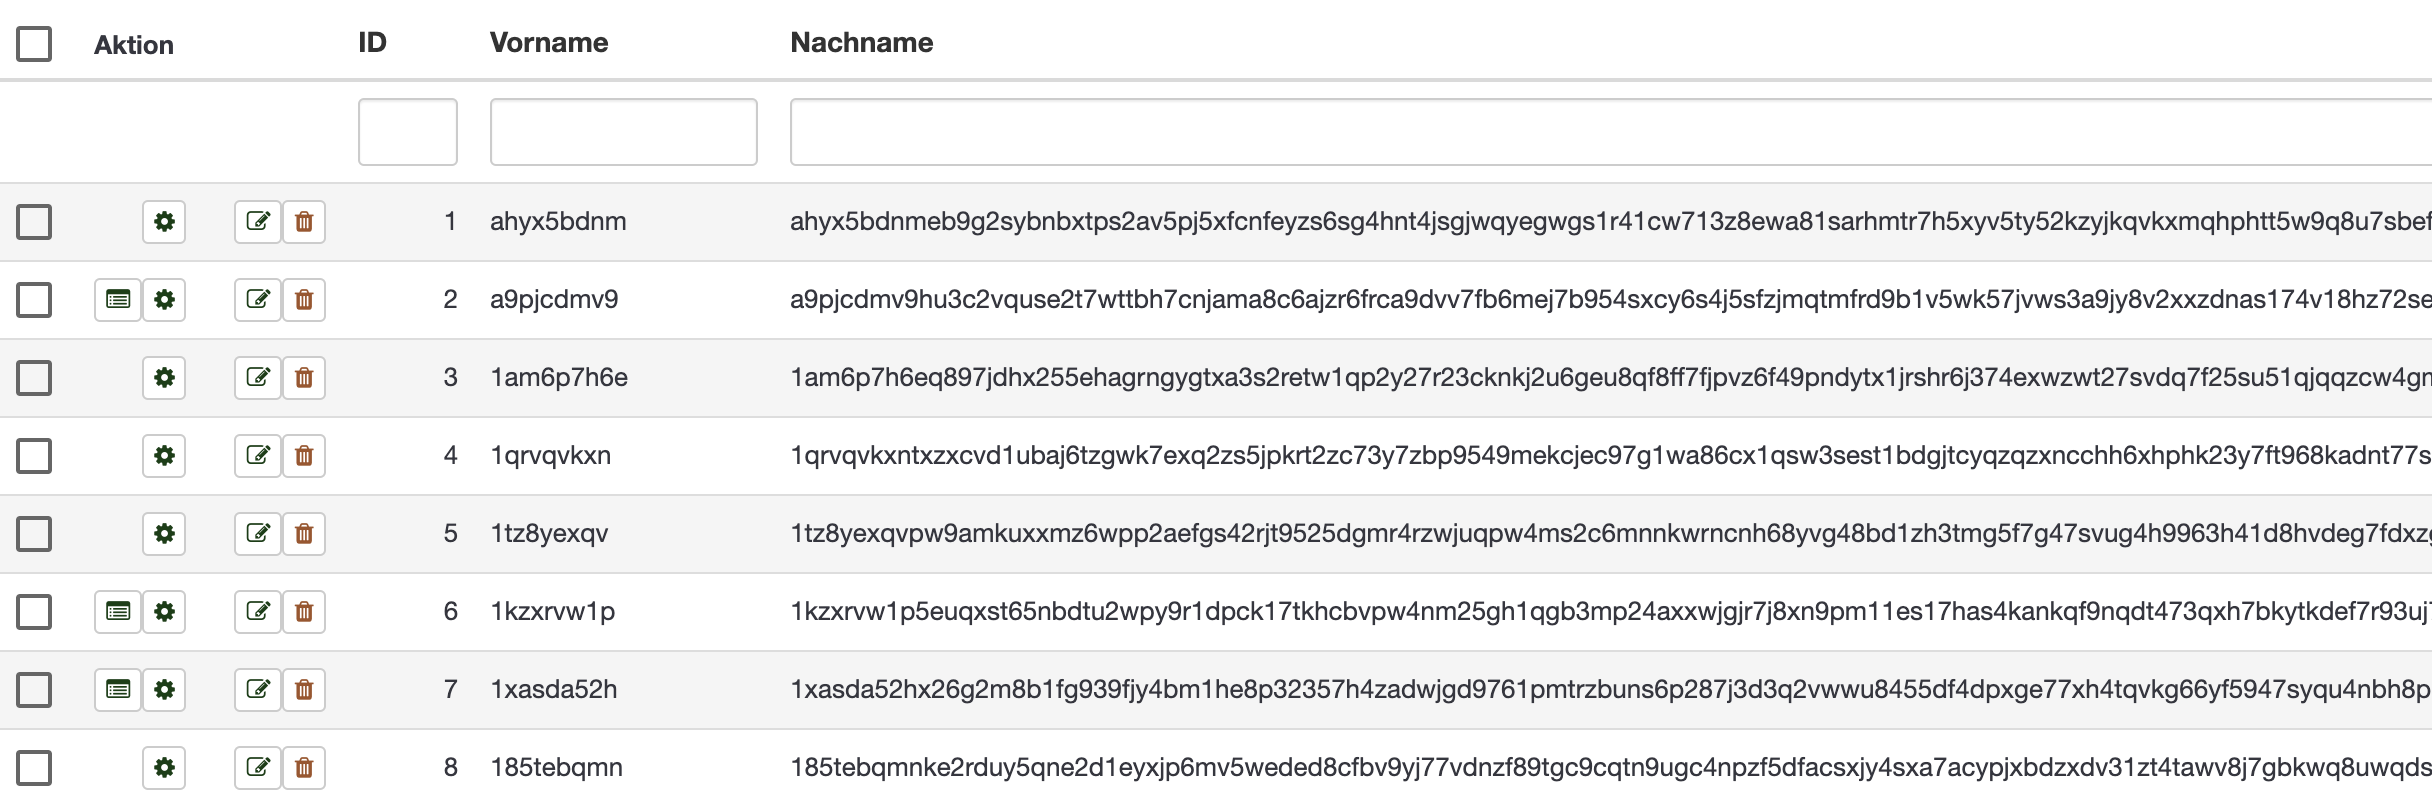
\includegraphics[width=1.0\textwidth]{docs/fig/ls_pseudonyms.png}
\end{figure}


\par\noindent\rule{\textwidth\color{pniblue}}{0.4pt}
\subsection*{Step 2. Entering the long ID in ALIIAS}
\addcontentsline{toc}{subsubsection}{Entering long ID in ALIIAS}

Connect the hardware key and start ALIIAS (see Step 1 in section \ref{section:sop_aliias}) and select 'Re-Identify' in the top menu bar. 
Paste the long ID to the dedicated input field and click the button "Re-identify" at the bottom.

\vspace{1mm}

\small\setlength\fboxsep{5pt}\setlength\fboxrule{1pt}
\fcolorbox{pniblue}{pniblue!5}{\begin{minipage}{0.9\textwidth}
Make sure there is no whitespace or other character copied to the clipboard together with the long ID.
\end{minipage}}

\vspace{1mm}

\small\setlength\fboxsep{5pt}\setlength\fboxrule{1pt}
\fcolorbox{pniblue}{pniblue!5}{\begin{minipage}{0.9\textwidth}
Logging in into ALIIAS with the LimeSurvey login is not necessary for re-identification.
\end{minipage}}
\large

\begin{figure}[H]
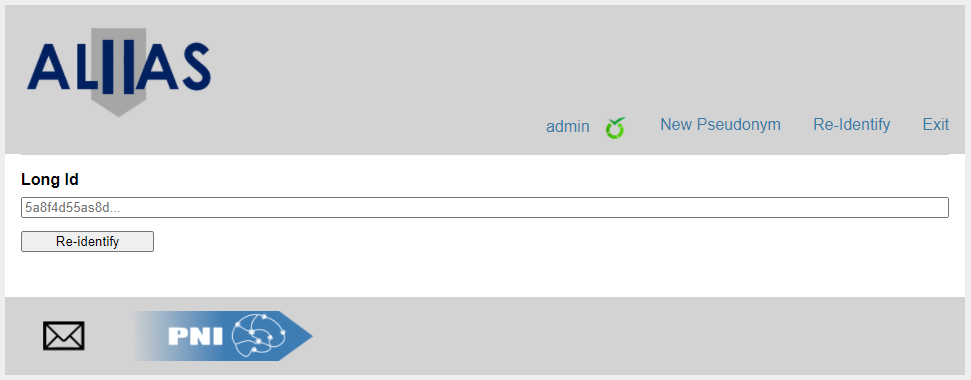
\includegraphics[width=0.9\textwidth]{docs/fig/06_reidentify.PNG}
\end{figure}

\subsection*{Step 2. Obtaining personal data}
\addcontentsline{toc}{subsubsection}{Obtaining personal data}

After clicking the "Re-identify" button, ALIIAS displays the personal data of the subject (on a panel with blue background).

The personal data of the subject can be used for obtaining the participant's contact details from the local 'participant list' (see section \ref{section:overview} for more details).

ALIIAS must be exited by clicking the "Exit" menu point in the top menubar, also as described in Step 7 of section \ref{section:sop_aliias}

\begin{figure}[H]
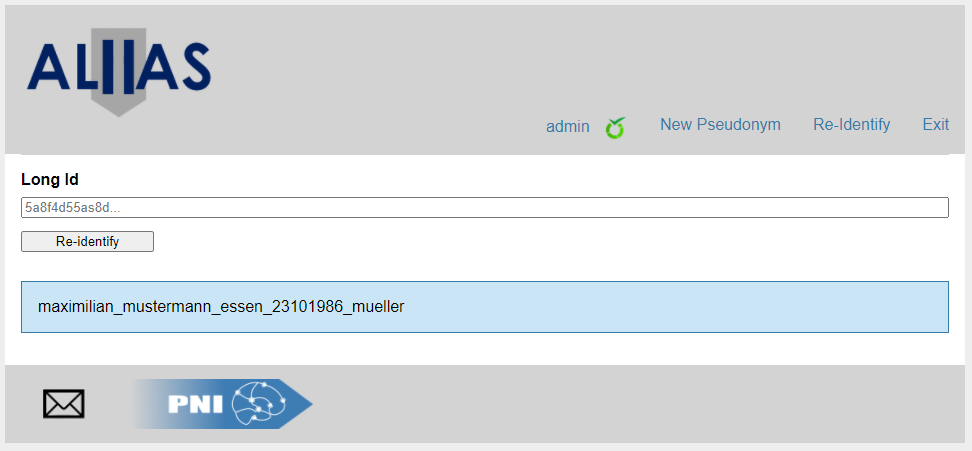
\includegraphics[width=0.9\textwidth]{docs/fig/07_reidentify_result.PNG}
\end{figure}
